\documentclass[12pt]{article}
\usepackage{tikz}
\usepackage{amsmath}
\usepackage{float}
\usepackage{caption}
\usepackage{array}
\usepackage{cancel}

\title{Simple\\Subtraction\\Course\\
\begin{center}

\includegraphics[width=4em]{ApS_logo.png}
\end{center}
\begin{normalsize}Tutoring Centre Ferndale \end{normalsize}}
\author{}
\date{\today}

\begin{document}
\maketitle

\section*{Subtraction}

Subtraction means taking away.\\

Subtraction is the opposite of addition.\\

To subtract a number is to take it away from some other number.\\

The subtraction of three things $\otimes\otimes\otimes$ from five things $\otimes\otimes\otimes\otimes\otimes$ leaves only two things $\otimes\otimes$.\\

\newpage

\begin{enumerate}

\item What is subtraction, in your own words?
\item What does it mean to subtract a number from another number?
\item If you subtract 5 things from 8 things, how many things are left?

\subsection*{Minus}
Minus means take away.\\

The minus symbol $-$ is used in writing subtraction.\\

$8-5=3$ means you are subtracting 5 from 8 leaving 3.

\item What does minus mean, in your own words?
\item Make a sentence that uses the word 'minus.'

\subsection*{Difference}
When you add numbers the result is called their sum or their total. When you subtract two numbers the result is called their difference. It is how different the two numbers are from each other.\\

Subtraction is written as:

\begin{table}[H]
    \centering
    \begin{tabular}{ccccc}
     \   & minus  &   \    & equals &  \ \\
     \large{8}    &  \large{$-$}    &   \large{3}    &   \large{=}    &  \large{5} \\
   number      &  \     &  number      &   \    & difference
    \end{tabular}
\end{table}

\newpage

\section*{Number Lines}
You can see what is happening on a number line. Moving to the right on the line represents adding, and moving to the left on the line represents subtracting.\\

Here is $2+3=5$:

\begin{center}
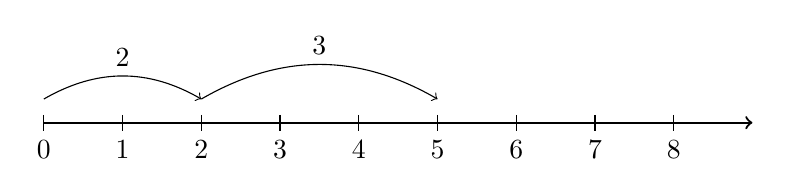
\begin{tikzpicture}
\draw[thick, ->] (0,0) -- (9,0) node[below] {$\ $};
\foreach \n in {0,1,2,3,4,5,6,7,8} {\draw (\n,0.1) -- (\n,-0.1) node[below] {$\n$};}
\draw[->, bend left=30] (0,0.3) to node[above] {$2$} (2,0.3);
\draw[->, bend left=30] (2,0.3) to node[above] {$3$} (5,0.3);
\end{tikzpicture}
\end{center}

And here is $5-3=2$:

\begin{center}
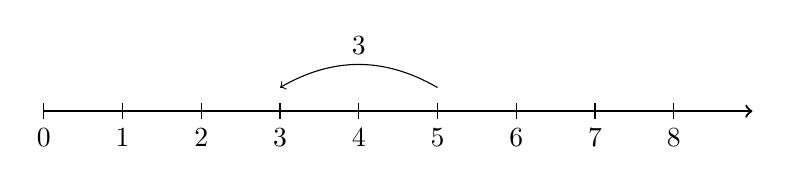
\begin{tikzpicture}
\draw[thick, ->] (0,0) -- (9,0) node[below] {$\ $};
\foreach \n in {0,1,2,3,4,5,6,7,8} {\draw (\n,0.1) -- (\n,-0.1) node[below] {$\n$};}
\draw[<-, bend left=30] (3,0.3) to node[above] {$3$} (5,0.3);
\end{tikzpicture}
\end{center}

\section*{Rearranging Addition}
Subtraction is the opposite of Addition. If you know your addition table for single-digit numbers then you also know how to subtract them because it's just the same numbers in a different order.

\begin{center}
$5 + 3 = 8$, so $8 - 3 = 5$
\end{center}

\item $7+2=9$, so what is 9-2?
\item $11+4=15$, so what is 15-4?
\item $3+2=5$, so what is 5-3?
\item $12+2=14$, so what is 14-2?
\item $8+6=14$, so what is 14-6?

\section*{The Subtraction Table}
Just like you learned the addition table, you should learn the subtraction table.

\begin{table}[h]
\centering
\begin{tabular}{|l|l|l|l|l|l|l|l|l|l|}
\hline
- & 1 & 2 & 3 & 4 & 5 & 6 & 7 & 8 & 9 \\ \hline
1 & 0 & . & . & . & . & . & . & . & . \\ \hline
2 & 1 & 0 & . & . & . & . & . & . & . \\ \hline
3 & 2 & 1 & 0 & . & . & . & . & . & . \\ \hline
4 & 3 & 2 & 1 & 0 & . & . & . & . & . \\ \hline
5 & 4 & 3 & 2 & 1 & 0 & . & . & . & . \\ \hline
6 & 5 & 4 & 3 & 2 & 1 & 0 & . & . & . \\ \hline
7 & 6 & 5 & 4 & 3 & 2 & 1 & 0 & . & . \\ \hline
8 & 7 & 6 & 5 & 4 & 3 & 2 & 1 & 0 & . \\ \hline
9 & 8 & 7 & 6 & 5 & 4 & 3 & 2 & 1 & 0 \\ \hline
\end{tabular}
\caption*{The Subtraction Table}
\end{table}

\item Fill in this blank subtraction table:\\

\begin{table}[ht]
\centering
\begin{tabular}{|l|l|l|l|l|l|l|l|l|l|}
\hline
- & 1 & 2 & 3 & 4 & 5 & 6 & 7 & 8 & 9 \\ \hline
1 &  & . & . & . & . & . & . & . & . \\ \hline
2 &  &  & . & . & . & . & . & . & . \\ \hline
3 &  &  &  & . & . & . & . & . & . \\ \hline
4 &  &  &  &  & . & . & . & . & . \\ \hline
5 &  &  &  &  &  & . & . & . & . \\ \hline
6 &  &  &  &  &  &  & . & . & . \\ \hline
7 &  &  &  &  &  &  &  & . & . \\ \hline
8 &  &  &  &  &  &  &  &  & . \\ \hline
9 &  &  &  &  &  &  &  &  &  \\ \hline
\end{tabular}
\caption*{Blank Subtraction Table}
\end{table}

\newpage

\section*{Subtraction in Columns}

Subtracting multi-digit numbers is done by arranging the numbers into columns aligned with the place-values all under each other. The ones, tens, hundreds and so on of each number should be under each other in vertical lines. Each column of digits is subtracted separately to get a difference that is written underneath.

For example, $72 - 21$ is $7 - 2 = 5$ for the tens digit, and $2 - 1 = 1$ for the ones digit, so that the difference is 51:

\begin{center}
\begin{tabular}{c@{\,}c@{\,}c@{\,}}
 &7&2\\
$-$&2&1\\
\hline
=&5&1\\
\hline
\hline
\end{tabular}
\end{center}

The difference is separated from the numbers by a single line, and is double underlined to show that this is a final answer.\\

Numbers, of any length, can be subtracted in this way, with the units, tens, thousands, and so on all aligned into columns to make the operation clear and simple.

\begin{center}
\begin{tabular}{c@{\,}c@{\,}c@{\,}c@{\,}c@{\,}c@{\,}c@{\,}c@{\,}}
  & &1&0&4,&2&1&3\\
 -& & & &3,&1&1&2\\
\hline
= & &1&0&1,&1&0&1\\
\hline
\hline
\end{tabular}\\
\end{center}

\item Subtract, in columns, 34 from 72.
\item Subtract, in columns, 4523 from 6721.

\newpage

\subsection*{Borrowing}
If the digit being subtracted is greater than the digit that it is being subtracted from then you have to borrow 10 from the digit to the left. You cross it out, replace it with 1 less, and write a small 1 to the left of the digit being subtracted from. That adds 10 so that the digits can now be subtracted properly.\\

Here, in the ones column, you can't take 5 from 3 so you borrow from the tens column. Cross out the 5 and make it a 4, and add that 10 to the 3 that now becomes 13. Now you can do $13-5=8$ for the ones digit and $4-1=3$ for the tens digit to get the difference as 38.

\begin{center}
\begin{tabular}{c@{\,}c@{\,}c@{\,}c@{\,}c}
& & &\(^{4}\)\cancel{5}&\(^{1}\)3\\
   - & & &1&5\\
	\hline
	& & &3&8\\
	\hline
	\hline
\end{tabular}
\end{center}

Here is another longer example of subtraction with borrowing:

\begin{center}
\begin{tabular}{c@{\,}c@{\,}c@{\,}c@{\,}c}
&\(^2\)\cancel{3},&\(^{13}\)\cancel{4}&\(^{14}\)\cancel{5}&\(^{1}\)6\\
   - & &7&8&9\\
	\hline
	&2,&6&6&7\\
	\hline
	\hline
\end{tabular}
\end{center}

\newpage

\subsubsection*{Chains of Borrowing}
If the digit to the left is zero so that you can't borrow from it, then you do a chain of borrowing from the next digit to the left so that the subtraction can still be done. You can carry from all the way across a long number this way if you have to.

Here we borrowed from all the way from the 1 at the left of a number to make the next digit a 10, then borrowed from that digit by making it a 9, and kept borrowing it like that all the way across to the ones digit.

\begin{center}
\begin{tabular}{c@{\,}c@{\,}c@{\,}c@{\,}c}
&\(^0\)\cancel{1},&\(^{9}\)\cancel{{\(^{1}0\)}}&\(^{9}\)\cancel{{\(^{1}0\)}}&\(^{1}0\)\\
   - & &7&8&9\\
	\hline
	&2,&6&6&7\\
	\hline
	\hline
\end{tabular}
\end{center}

\section*{Practice:}

\item What is 742 - 389?
\item What is 956 - 417?
\item What is 820 - 398?
\item What is 574 - 289?
\item What is 643 - 326?
\item What is 968 - 537?
\item What is 726 - 398?
\item What is 800 - 476?
\item What is 921 - 582?
\item Keep practicing subtracting numbers until you are getting right answers every time and you feel confident about it.\\

And that's how you do subtraction!

\newpage

\section*{Adding and Subtracting\\by Equal Adjustment}
Sometimes when adding or subtracting two numbers it is easier to add or subtract a small amount to both numbers, to make the units digit equal to zero. You don't have to carry or borrow digits this way, which is easier, and with practice you can do it in you head without writing.\\

\subsection*{Adding}
For example, $78 + 96$ is the same as $78 + 2 + 96 - 2$. You are just adding two and taking it away again, leaving the sum unchanged. It is easier to add $80 + 94$ than to add $78 + 96$, but they both result in the same sum.

Add these numbers by adjusting:
\item 348 + 52
\item 176 + 124
\item 637 + 363

\subsection*{Subtracting}
In the same way, $96 - 78$ is the same as $96 + 2 - 78 + 2$. The difference remains the same. $98 - 80$ is a much easier problem to solve.

Subtract these numbers by adjusting:
\item 723 - 323
\item 957 - 457
\item 826 - 326

\end{enumerate}

Practice subtracting all sorts of numbers until you can do it easily and get it right every time!

\end{document}
